\subsection{GFP}
    \label{section:gfp}
    Green fluorescent protein (GFP) is protein that produces bright green fluroescence from the whole cell surface. Some cells express this protein naturally, therefore there is no need to perform cell staining or fixation in this case and the imaging can be done on living cells. Fixation of the cells is a processes of destructing their membrane and fixing them on the plate in order for the stain antibody to be able to enter the cell. The difference in DIC imaging between fixed and not fixed cells is presented in Figure \ref{fig:fixed-not-fixed}. Clearly, cell membrane is intact and clearly defined in not fixed cells, whereas in not fixed ones there is almost no definite membrane present. 
    
    Nevertheless, in order to get training data for all other targets (nuclei, ER, Golgi apparatus) the staining procedure is unavoidable. And staining requires the cells first to be fixed. That brings up the limitation of current \textit{in silico} labeling research --- cells have to be fixated in any case. DIC imaging of living and fixed cells look very different and models trained on fixed cells do not generalize well to not fixed ones. Luckily, fixing cells is not a cumbersome lab procedure and is far easier than staining the cells, which is escaped with the help of \textit{in silico} fluorescence labeling. After successfull training of the model on living GFP expressing cells, we found out that other models cannot perform that well on living cells. Therefore, the cells were fixed in order to look alike with previously acquired data and the experiments were repeated. Nevertheless, we recommend to look into the possibilities of transfer learning from fixed to live cells. The results of training on the fixated cells are presented below. 
    
    For this experiment another cell phenotype was chosen --- H19. Training the model to predict GFP fluorescence essentially allows to predict the area of the whole cell, that is used in further downstream analysis. There is no need to capture the intensities as they do not bring any useful features for selection step in CLD. However they might help for algorithms like watershed to find separate cells in order to count them. Yet the task can be simplified to predicting binary mask of GFP signal too. Binarized images are well-suited for cell area predictions. Altough one has to find a corresponding image preprocessing pipeline in order to convert training intesity fluorescence imaging into masks first. Both tranining variations are provided in this chapter --- with and without prediction of the intensities. 
    \begin{figure}[H]
        \begin{center}
            \includegraphics[width=0.5\linewidth]{bilder/gfp/fixed-not-fixed.png}
            \caption{Examples of fixed and not fixed cells DIC imaging}\label{fig:fixed-not-fixed}
        \end{center}
    \end{figure}
    \subsubsection{Preprocessing}
        \begin{figure}[H]
	\begin{center}
		\includegraphics[width=0.5\linewidth]{bilder/gfp/binary-bce/preprocessing/preprocessing-gfp.png}
		\caption{Converting GFP to a binary mask}\label{fig:gfp-binary}
	\end{center}
\end{figure}

    \subsubsection{Predictions}
        \begin{figure}[htb]
	\begin{center}
		\includegraphics[width=0.8\linewidth]{bilder/gfp/binary-bce/enlarged.png}
		\caption{Binary training with BCE}\label{fig:gfp-bce-predictions}
	\end{center}
\end{figure}

\begin{figure}[htb]
	\begin{center}
		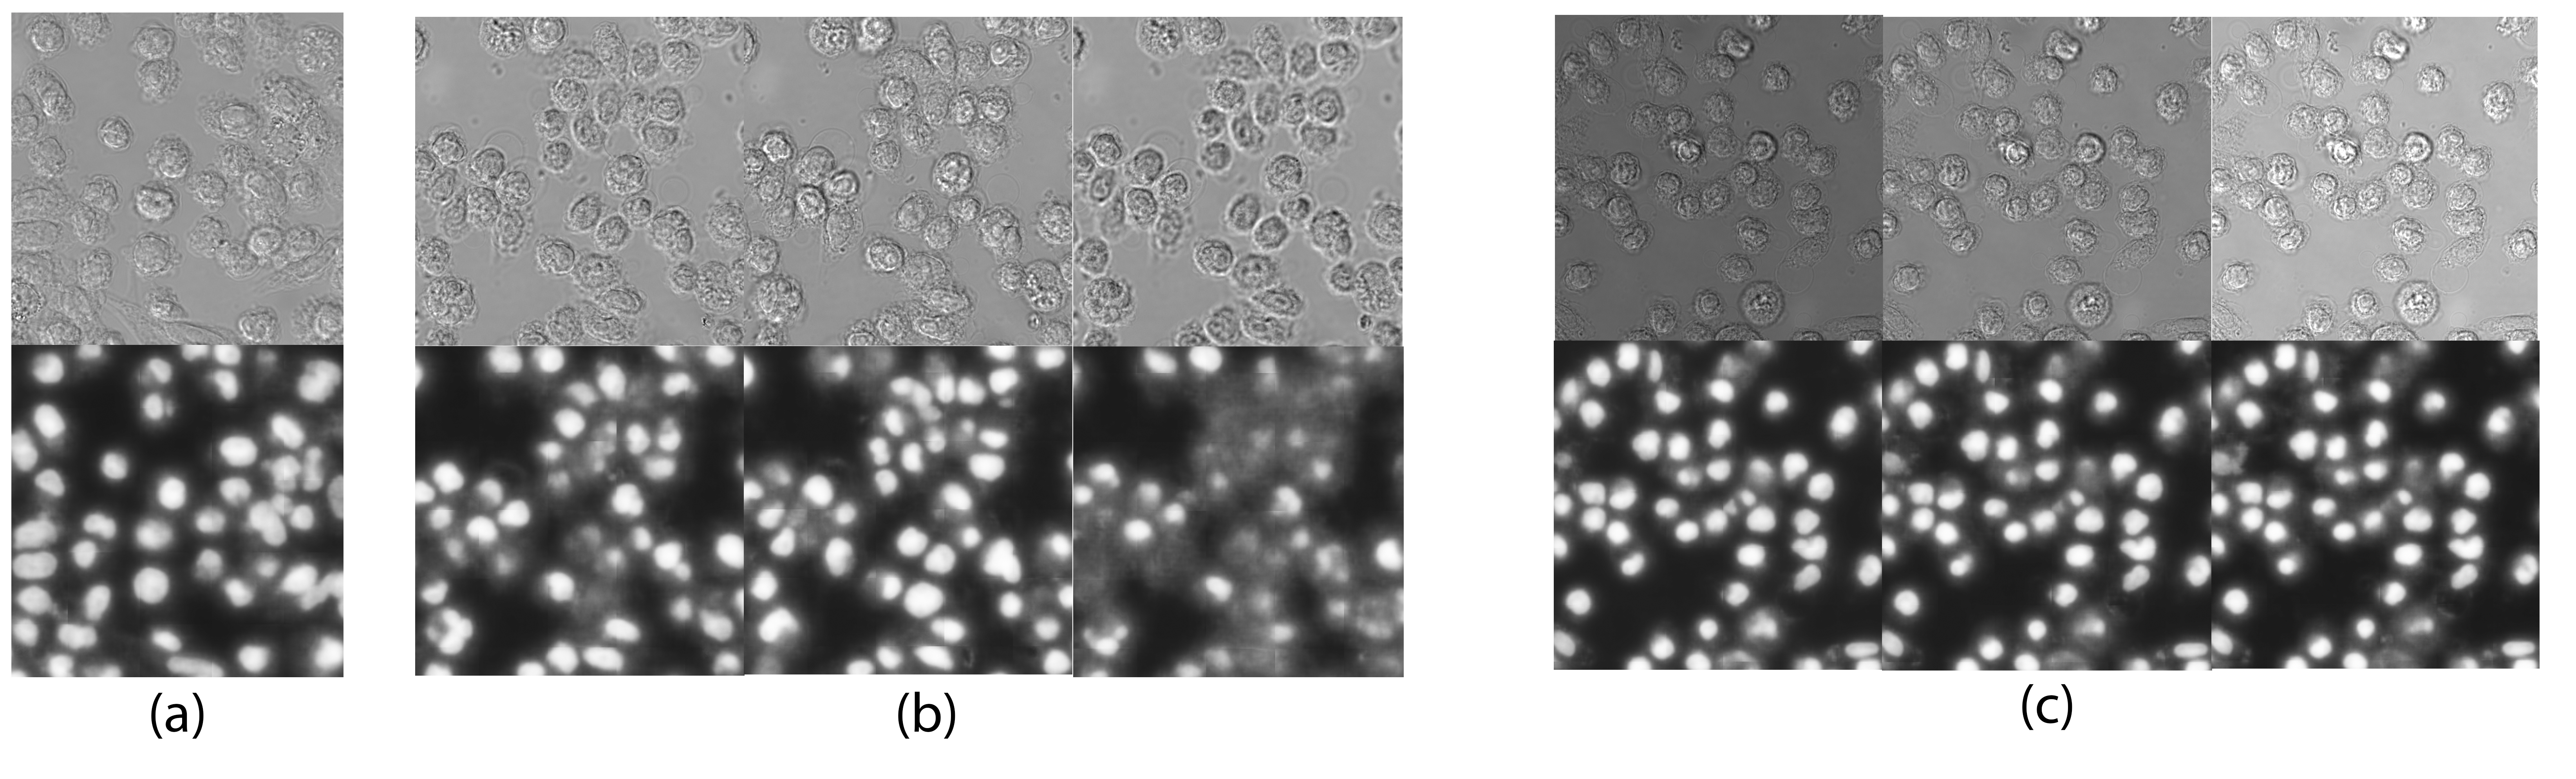
\includegraphics[width=0.6\linewidth]{bilder/gfp/predictions.png}
		\caption{Training with Pearson correlation loss}\label{fig:gfp-pcc-predictions}
	\end{center}
\end{figure}

\begin{table}[H]
    \centering
    \caption{Correlation coefficients for downstream tasks}
        \begin{adjustbox}{width=0.4\textwidth}
            \begin{tabular}{|c|c|c|}\hline
                Binary training&Pearson&Spearman
                \\\hline\hline
                Number of ER&0.67&0.64\\\hline
                Area&0.82&0.75\\\hline\hline
                Continuos training&Pearson&Spearman\\\hline
				Number of ER&0.57&0.55\\\hline
                Area&0.26&0.64\\\hline
            \end{tabular}
        \end{adjustbox}
\end{table}

    \subsubsection{Downstream metrics}
        TODO move to separate chapter?
        \begin{figure}[H]
	\begin{center}
		\includegraphics[width=\linewidth]{bilder/gfp/binary-bce/gfp-bce-metrics.png}
		\caption{Downstream metrics}\label{fig:gfp-bce-metrics}
	\end{center}
\end{figure}
    \subsubsection{Combination of GFP, nuclei and ER}
        Now having three successfull models that are able to prediction GFP fluorescence from the whole cell, nuclei and ER, one can combine their predictions together for the same image. For that an output RGB image was contructed, where each prediction takes one channel. In this case channel correspondence is the following: red --- ER, green --- GFP, blue --- nuclei. The resulting image is shown in Figure \ref{fig:combined}. Additionally one can see, that GFP model has successfully generalized on other cell phenotypes (CHOZN, PHX), although it was train on H19 only.
\begin{figure}[htb]
	\begin{center}
		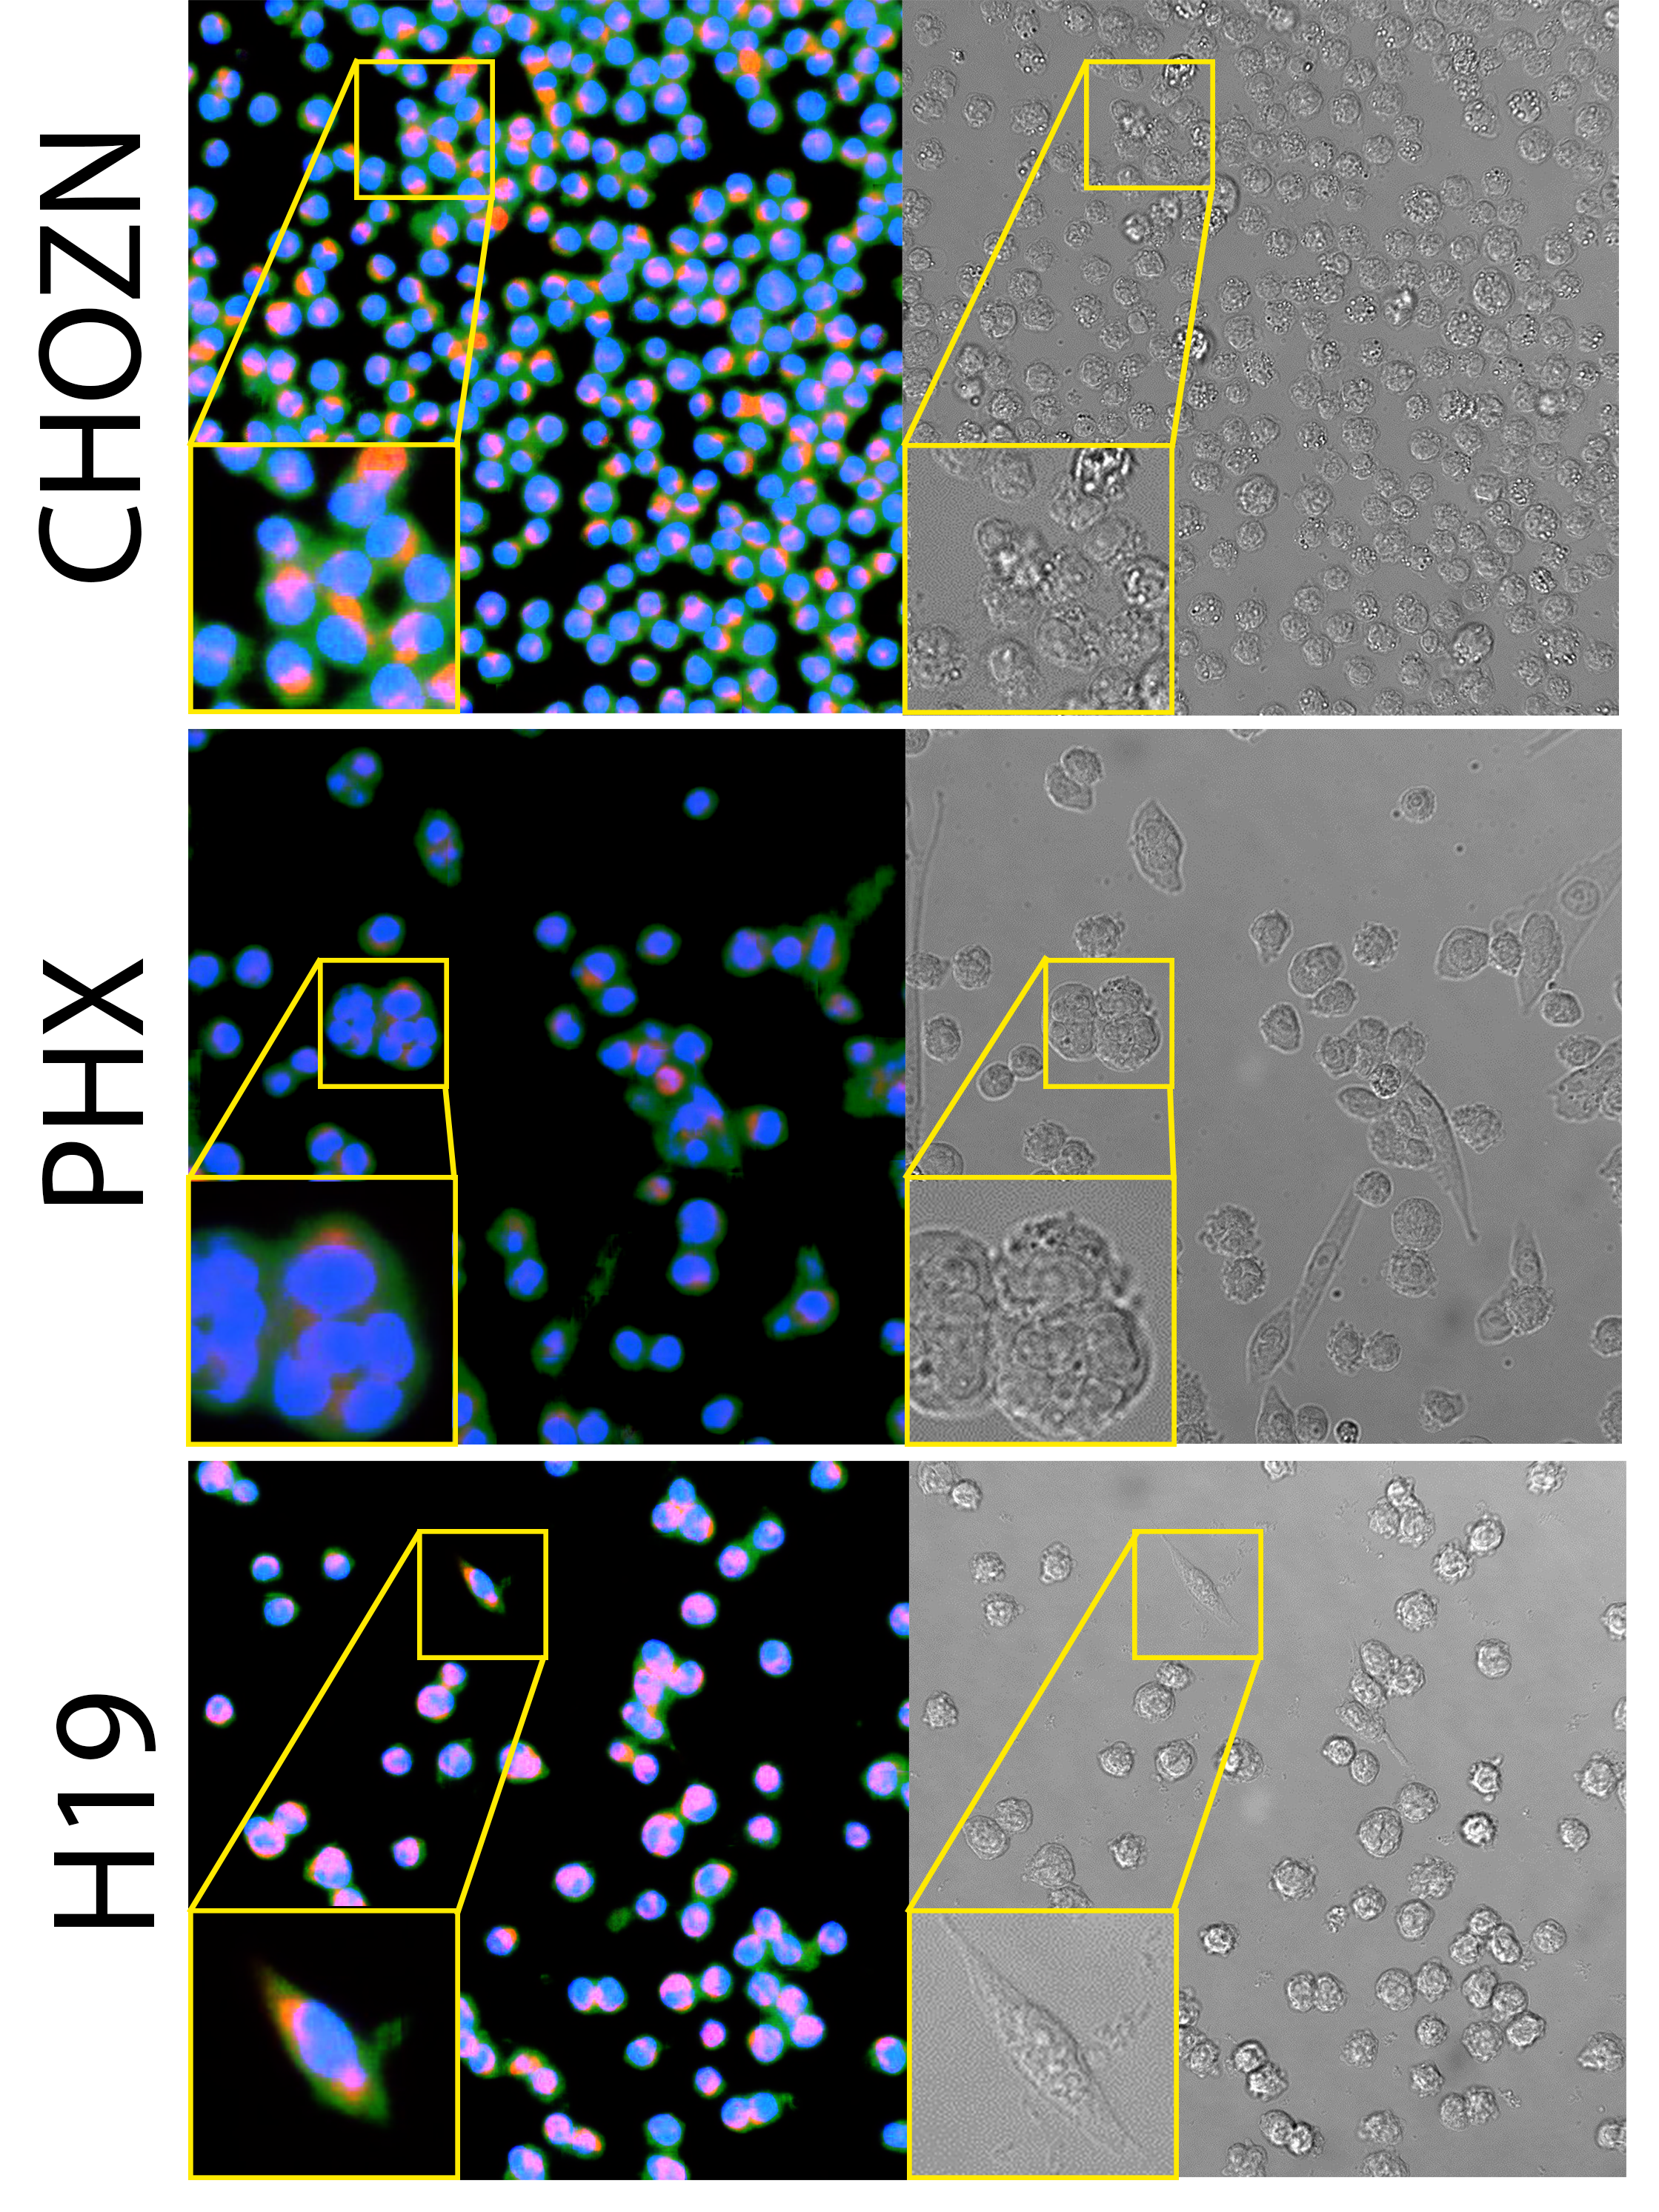
\includegraphics[width=0.4\linewidth]{bilder/combined/combined.png}
		\caption{GFP, Nuclei and ER combined}\label{fig:combined}
	\end{center}
\end{figure}

    \subsubsection{Conclusions}
        GFP \textit{in silico} fluorescence labeling can successfully be used for counting number of cells and estimating their size. The created models can both predict the intensity images as well as binarized masks. Intensity predictions might be more useful for number of cell estimation as the cells separate there visually better. The models was evaluated on two donstream metrics: cell size and cell count. Correlation coefficient suggest a strong correlation between the predictions and ground truth. The model has limitation in its diability to differentiate between dead and alive cells. This issue should be addressed in further reasearch after acquiring data for labeling dead cells. Despite the difficulty of clear determination of cell boundary during image preprocessing for fluorescence image binarization (its overprediction in some cases) the model can successfully generalize and predict a correct boundary for all cells. The images of not fixed cells were provided for the first time during GFP experiments and it was clear that previously trained model do not generalize on them well, therefore the limitation of research in terms of the cell fixation need was determined. However, its recommened to look into possible transfer learning approaches to get rid of fixation step completely.
  
